\documentclass[xcolor=dvipsnames,aspectratio=169]{beamer}

% INCLUSIÓN DOS PAQUETES IMPRESCINDIBLES DE IDIOMA E CODIFICACIÓN DE CARACTERE.
\usepackage[T1]{fontenc}
\usepackage[english]{babel}
\usepackage[utf8]{inputenc}
\usepackage{csquotes}

%ACRONYMS para engadir un glosario de acronimos automatizado
% \usepackage[acronyms,nonumberlist,nopostdot,nomain,nogroupskip]{glossaries}
% \input{./acronyms.tex}

% PAQUETES PARA FIGURAS E GRAFICOS
\usepackage{graphicx}
%   \usepackage[pdftex]{graphicx}
  \usepackage{epstopdf}
   \graphicspath{{./img/}}
  % and their extensions so you won't have to specify these with
  % every instance of \includegraphics
   \DeclareGraphicsExtensions{.eps,.pdf,.png,.jpg}   
\usepackage{subfigure}
\usepackage{caption}
\usepackage[inkscapelatex=false]{svg}

%Tikz plots
\usepackage{tikz}
\usepackage{tikzscale}
\usetikzlibrary{plotmarks,patterns,decorations.pathreplacing,backgrounds,calc,arrows,arrows.meta,spy,matrix,backgrounds,shapes,math}

\tikzset{
    block/.style = {draw, rectangle, 
        minimum height=1cm, 
        minimum width=1.2cm, align=center},
    input/.style = {coordinate,node distance=1cm},
    output/.style = {coordinate,node distance=2cm},
    arrow/.style={draw, -latex,node distance=1.5cm},
    pinstyle/.style = {pin edge={latex-, black,node distance=1.5cm}},
    sum/.style = {draw, circle, node distance=1cm}
}

\newcommand{\tikzmark}[1]{\tikz[overlay,remember picture] \UE (#1) {};}
\newcommand{\DrawBox}[4][]{%
    \tikz[overlay,remember picture]{%
        \coordinate (TopLeft)     at ($(#2)+(-0.4em,1.6em)$);
        \coordinate (BottomRight) at ($(#3)+(0.4em,-1.0em)$);
        %
        \path (TopLeft); \pgfgetlastxy{\XCoord}{\IgnoreCoord};
        \path (BottomRight); \pgfgetlastxy{\IgnoreCoord}{\YCoord};
        \coordinate (LabelPoint) at ($(\XCoord,\YCoord)!0.5!(BottomRight)$);
        %
        \draw [red,#1] (TopLeft) rectangle (BottomRight);
        \UE [below, #1, fill=none, fill opacity=1] at (LabelPoint) {#4};
    }
}
\usepackage{pgfplots}
\pgfplotsset{compat=newest}
\pgfplotsset{plot coordinates/math parser=false}
\usepgfplotslibrary{patchplots,groupplots}

\tikzstyle{pinstyle} = [pin edge={to-,thin,black}]
\def\antenna{%
    -- +(0mm,4.0mm) -- +(2.625mm,7.5mm) -- +(-2.625mm,7.5mm) -- +(0mm,4.0mm) -- +(0mm,0mm)
}


% OUTROS PAQUETES DE USO COMUN. HOXE EN DIA OS COMPILADORES SON TAN RAPIDOS QUE EU METO TODOS SEMPRE
% \usepackage{float}
% \usepackage{ucs} 
% \usepackage{subcaption}
\usepackage{psfrag}
\usepackage{verbatim}
\usepackage{amsmath}
\usepackage{amsfonts} 
\usepackage{amssymb} 
\usepackage{amsthm}
\usepackage{pifont}
\usepackage{array}
\usepackage{listings}
\usepackage{stfloats}
\usepackage{algorithm} 
\usepackage{algorithmic} 
\usepackage{url} 
\usepackage{enumerate}
\usepackage{multirow}
\usepackage{wasysym}
\usepackage{cancel}
\usepackage{lmodern}

\usepackage{mathrsfs}  

% DECLARACION DAS FONTES DA UVIGO
\usepackage[sfdefault]{roboto}
\usepackage{librebaskerville}
\setbeamerfont{title}{family=\librebaskerville,size=\Huge}
\setbeamerfont{subtitle}{family=\librebaskerville,size=\large}
% IMPORTANTE: a fonte 'campus' non queda ben para títulos de papers academicos,ç
% pero se de verdade se desexa empregar, seguir os seguintes pasos
% 1) Instalar o comando otftotfm en linux
% 2) sudo otftotfm -a -e texnansx campus_bold.otf CampusBold
% 3) asegurarse que o ficheiro auxiliar ./EETtemplateFiles/fonts/T1CampusBold.df está no directorio de traballo
% 4) descomentar a liña abaixo e comentar a liña que lle asigna librebaskerville arriba
\input{EETtemplateFiles/fonts/T1CampusBold.df}
\setbeamerfont{title}{family=\fontfamily{CampusBold},size=\Huge}

% DETLARACIÓN DO TEMA A USAR
% 
% ESTES TEMAS TEÑEN CABECEIRAS MOI GRANDES
% \usetheme{Berkeley} %large titlebar w/side dossier
% \usetheme{PaloAlto} 
% \usetheme{Copenhagen} %large titlebar w/2 side index
% \usetheme{Antibes} %large titlebar w/tree
% \usetheme{Singapore} %large titlebar w/balls evanescent
% \usetheme{Berlin} %large titlebar w/balls solid
% \usetheme{Dresden} %same as above with different color boxing
% \usetheme{Rochester} %large tittle-only titlebar
% ESTES TEMAS TEÑEN CABECEIRAS MEDIANAS
% \usetheme{CambridgeUS} %title titlebar w/current section
% \usetheme{Malmoe} %title titlebar w/current section Copenhagen style
% \usetheme{Madrid} %title titlebar w/page counter footer
% ESTES TEMAS TEÑEN CABECEIRAS DELGADAS
% \usetheme{Frankfurt} %small titlebar w/ progress balls
% \usetheme{metropolis} %metal
% ESTES TEMAS NON TEÑEN CABECEIRA DE COR, PERO SI TITULO SOBRE BRANCO
% \usetheme{Boadilla} %sombras e decoracion
\usetheme{Pittsburgh} %rectangulos planos
% ESTES TEMAS TEÑEN INDICES OU INFO NUNHA BARRA LATERAL GRANDE
% \usetheme{Goettingen} %right dossier evanescent
% \usetheme{Marburg} %right dossier fading to black
% \usetheme{Bergen} %notebook

%aspect modifiers
\useinnertheme{circles} %this makes item lists nicer
% \useoutertheme{infolines} %toggle thin info borders


% DECLARACIÓN DA COMBINACIÓN DE CORES A USAR. SE NON SE ESPECIFICA NADA TOMA A DEFINIDA POR DEFECTO
\definecolor{EETblue}{HTML}{0094e0} % a mate dark blue
\usecolortheme[named=EETblue]{structure} % EET UVigo blue
% outros temas de cores de beamer
% \usecolortheme{seagull} %makes title boxes gray color with blackr
% \usecolortheme{spruce} %makes title boxes pastel blue - gray color
% cores internos (items)
% \usecolortheme[named=Red]{structure} 
% \usecolortheme[named=Green]{structure} 
% \usecolortheme[named=OliveGreen]{structure} 
% \usecolortheme[named=PineGreen]{structure} 
% \usecolortheme[named=TealBlue]{structure} 
% \usecolortheme[named=SeaGreen]{structure}
% \usecolortheme[RGB={00,78,135}]{structure} % a dark cobalt blue 
% \usecolortheme[RGB={155,0,20}]{structure} % a slighlty darkened mate red

% MODIFICACIONS DAS CORES PARA A PAXINA DE TITULO SIMILAR Á OFICIAL
\setbeamercolor*{title}{use=structure,fg=structure.bg, bg=structure.fg}  
\setbeamercolor*{subtitle}{use=structure,fg=white}  
\setbeamercolor*{author}{use=structure,fg=structure.fg}
% \setbeamercolor*{institute}{use=structure,fg=structure.fg}
\setbeamercolor*{date}{use=structure,fg=structure.fg}
\setbeamertemplate{frametitle}[default][left]

% MODIFICACIONS DA SIDEBAR E FOOTLINE PARA INCLUIR AS IMAXES CORPORATIVAS.
\setbeamertemplate{footline}[text line]{%
  \parbox{\linewidth}{
    %ESTE TEXTO DA FOOTLINE PODESE MODIFICAR A GUSTO -----------------------------------------
    \insertshorttitle\hfill\insertshortauthor\hfill\insertpagenumber / \inserttotalframenumber
    %----------------------------------------------------------------------------------------
    \hfill
  
\includegraphics[width=.15\paperwidth,trim={0 2.5cm 3.5cm .75cm},clip]{EETtemplateFiles/img/Logotipo_ESCOLA.pdf}\vspace*{2pt}}}
\setbeamersize{sidebar width left = .10\paperwidth}
\setbeamertemplate{sidebar canvas left}{}
\setbeamertemplate{sidebar left}{%
  \vspace*{\fill}
  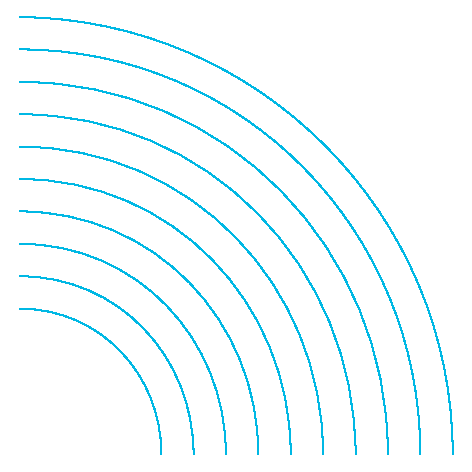
\includegraphics[width=.15\paperwidth,height=.15\paperwidth]{EETtemplateFiles/img/Simbolo_ESCOLA.pdf}\\
  
\includegraphics[width=.15\paperwidth,trim={.4cm .5cm .4cm 2.25cm},clip]{EETtemplateFiles/img/Logotipo_ESCOLA.pdf}
  \vspace*{-11pt}%
}

% MATH SYMBOLS

\newcommand{\field}[1]{\mathbb{#1}}

\DeclareMathOperator{\atan}{atan}
\DeclareMathOperator{\acos}{acos}
\DeclareMathOperator{\asin}{asin}

% \newcommand{\mb}[1]{\mathbf{#1}}


\newcommand{\A}{\mathbf{A}}
\newcommand{\B}{\mathbf{B}}
\newcommand{\Cb}{\mathbf{C}}
\newcommand{\D}{\mathbf{D}}
\newcommand{\Eb}{\mathbf{E}}
\newcommand{\F}{\mathbf{F}}
\newcommand{\Gb}{\mathbf{G}}
\newcommand{\Hb}{\mathbf{H}}
\newcommand{\I}{\mathbf{I}}
\newcommand{\J}{\mathbf{J}}
\newcommand{\Kb}{\mathbf{K}}
\newcommand{\Lb}{\mathbf{L}}
\newcommand{\M}{\mathbf{M}}
\newcommand{\N}{\mathbf{N}}
\newcommand{\Ob}{\mathbf{O}}
\newcommand{\Pb}{\mathbf{P}}
\newcommand{\Q}{\mathbf{Q}}
\newcommand{\R}{\mathbf{R}}
\newcommand{\Sb}{\mathbf{S}}
\newcommand{\T}{\mathbf{T}}
\newcommand{\U}{\mathbf{U}}
\newcommand{\V}{\mathbf{V}}
\newcommand{\W}{\mathbf{W}}
\newcommand{\X}{\mathbf{X}}
\newcommand{\Y}{\mathbf{Y}}
\newcommand{\Z}{\mathbf{Z}}
\newcommand{\Dl}{\mathbf{\boldsymbol{\Delta}}}
\newcommand{\Sg}{\mathbf{\boldsymbol{\Sigma}}}
\newcommand{\Ld}{\mathbf{\boldsymbol{\Lambda}}}
\newcommand{\Ph}{\mathbf{\boldsymbol{\Phi}}}
\newcommand{\Ps}{\mathbf{\boldsymbol{\Psi}}}
\newcommand{\Up}{\mathbf{\boldsymbol{\Upsilon}}}
\newcommand{\Xib}{\mathbf{\boldsymbol{\Xi}}}
% \newcommand{\D}{\mathbf{D}}
\newcommand{\one}{\mathbf{1}}
\newcommand{\zero}{\mathbf{0}}

\newcommand{\ab}{\mathbf{a}}
\newcommand{\bb}{\mathbf{b}}
\newcommand{\cc}{\mathbf{c}}
\newcommand{\dd}{\mathbf{d}}
\newcommand{\e}{\mathbf{e}}
\newcommand{\f}{\mathbf{f}}
\newcommand{\g}{\mathbf{g}}
\newcommand{\h}{\mathbf{h}}
\newcommand{\ib}{\mathbf{i}}
\newcommand{\jb}{\mathbf{j}}
\newcommand{\kb}{\mathbf{k}}
\newcommand{\lb}{\mathbf{\ell}}
\newcommand{\m}{\mathbf{m}}
\newcommand{\n}{\mathbf{n}}
\newcommand{\ob}{\mathbf{o}}
\newcommand{\pp}{\mathbf{p}}
\newcommand{\q}{\mathbf{q}}
\newcommand{\rr}{\mathbf{r}}
\newcommand{\s}{\mathbf{s}}
\newcommand{\uu}{\mathbf{u}}
\newcommand{\vv}{\mathbf{v}}
\newcommand{\w}{\mathbf{w}}
\newcommand{\x}{\mathbf{x}}
\newcommand{\y}{\mathbf{y}}
\newcommand{\z}{\mathbf{z}}
\newcommand{\al}{\mathbf{\boldsymbol{\alpha}}}
\newcommand{\vmu}{\mathbf{\boldsymbol{\mu}}}
\newcommand{\vlambda}{\mathbf{\boldsymbol{\lambda}}}
\newcommand{\vphi}{\mathbf{\boldsymbol{\phi}}}
\newcommand{\vpsi}{\mathbf{\boldsymbol{\psi}}}
\newcommand{\vrho}{\mathbf{\boldsymbol{\rho}}}
\newcommand{\vups}{\mathbf{\boldsymbol{\upsilon}}}
\newcommand{\vxi}{\mathbf{\boldsymbol{\xi}}}

\newcommand{\rank}{\textnormal{rank}}
% \newcommand{\trace}{\textnormal{trace}}
\newcommand{\exptr}{\textnormal{exptr}}
\newcommand{\tr}{\textnormal{tr}}
% \newcommand{\vstack}{\textnormal{vec}}
% \newcommand{\diag}{\textnormal{diag}}
\newcommand{\vstack}[1]{\Xib_{#1}}
\newcommand{\diag}[1]{\Ld_{#1}}
\newcommand{\tnsr}[2]{\underline{\mathsf{#1}}_{#2}}
\newcommand{\tmult}[1]{\underset{#1}{\times}}

\DeclareMathOperator{\Prob}{Prob}
%  |x>
\newcommand{\ket}[1]{\left\vert#1\right\rangle}
%  <x|
\newcommand{\bra}[1]{\left\langle#1\right\vert}
%  <x|y>
\newcommand{\braket}[2]{\left< #1 \vphantom{#2}\,
                        \right\vert\left.\!\vphantom{#1} #2 \right>}
%  <x|a|y>
\newcommand{\sandwich}[3]{\left< #1 \vphantom{#2 #3} \right|
                          #2 \min\left(\vphantom{#1 #2} #3 \right>}

\newcommand{\pd}[2]{\frac{\partial #1}{\partial #2}}
%  d/dt
\newcommand{\ddt}{\frac{d}{dt}}
%  D/Dx
\newcommand{\pdd}[1]{\frac{\partial}{\partial#1}}
%  |x|
\newcommand{\abs}[1]{\left\vert#1\right\vert}
%  k_{x}
\newcommand{\kv}[1]{\mathbf{k}_{#1}}
%  \textnormal{E}_{domain of integration}{variable}
\newcommand{\Ex}[2]{{\mathbb{E}_{#1}\left[#2\right]}}
\newcommand{\CEx}[3]{{\mathbb{E}_{#1}\left[#2|#3\right]}}
\newcommand{\CInf}[3]{{\textnormal{I}\left(#1;#2|#3\right)}}
\newcommand{\Inf}[2]{{\textnormal{I}\left(#1;#2\right)}}
\newcommand{\CEnt}[2]{{\textnormal{H}\left(#1|#2\right)}}
\newcommand{\Ent}[1]{{\textnormal{H}\left(#1\right)}}
\newcommand{\dCEnt}[2]{{\textnormal{h}\left(#1|#2\right)}}
\newcommand{\dEnt}[1]{{\textnormal{h}\left(#1\right)}}

\newcommand{\cmark}{\ding{51}}%
\newcommand{\xmark}{\ding{55}}%
\newcommand{\itempro}{\item[\textcolor{KYJade}{\Large \cmark}]}
\newcommand{\itemcontra}{\item[\textcolor{ARust}{\Large \xmark}]}
\newcommand\Tau{\mathcal{T}}
%Figure and format fixes


\renewcommand{\figurename}{Fig.}
\newcommand{\PESrule}{\noindent\rule{.57\columnwidth}{0.1mm}}

%theroem environments
% If using amsthm package, we need to delete these theorems before giving them our own definition. does not work for theorem
% \let\theorem\relax
\let\definition\relax
\let\lemma\relax
\let\corollary\relax
\let\example\relax
%
% \newtheorem{theorem}{Theorem}
\newtheorem{definition}{Definition}
\newtheorem{lemma}{Lemma}
\newtheorem{corollary}{Corollary}
\newtheorem{conjecture}{Conjecture}
\theoremstyle{plain}
\newtheorem{remark}{Remark}
\newtheorem{proposition}{Proposition}
\newtheorem{example}{Example}
\newtheorem{homework}{Homework}

%Colors
   \definecolor{blueH3}{rgb}{0,.5,1}
   \definecolor{blueH2}{rgb}{0,0.25,0.75}
   \definecolor{blueH1}{rgb}{0,0,0.5}   
   \definecolor{grayOldText}{rgb}{.5,.5,.5}
   \definecolor{VCobalt}{HTML}{005682}
   \definecolor{TZTeal}{HTML}{008080}
   \definecolor{TZTealfaded}{HTML}{F0FFFF}
   \definecolor{KYJade}{HTML}{008151}
   \definecolor{ARust}{HTML}{a10000}
   \definecolor{FFucsia}{HTML}{7000c3}   
   \definecolor{TAMustard}{HTML}{a1a100}
   \definecolor{Tangerine}{HTML}{d45500}
   
   
% Tikz 
% signal block diagram components
\tikzset{
    block/.style = {draw, rectangle, 
        minimum height=1cm, 
        minimum width=1.2cm, align=center},
    input/.style = {coordinate,node distance=1cm},
    output/.style = {coordinate,node distance=2cm},
    arrow/.style={draw, -latex,node distance=1.5cm},
    pinstyle/.style = {pin edge={latex-, black,node distance=1.5cm}},
    sum/.style = {draw, circle, node distance=1cm}
}
\tikzstyle{pinstyle} = [pin edge={to-,thin,black}]
\def\antenna{%
    -- +(0mm,4.0mm) -- +(2.625mm,7.5mm) -- +(-2.625mm,7.5mm) -- +(0mm,4.0mm) -- +(0mm,0mm)
}
% Overlay highlights on top of the page
\newcommand{\markOverlay}[1]{\tikz[overlay,remember picture] \node (#1) {};}
\newcommand{\drawOverlayBox}[4][]{%
    \tikz[overlay,remember picture]{%
        \coordinate (TopLeft)     at ($(#2)+(-0.4em,1.6em)$);
        \coordinate (BottomRight) at ($(#3)+(0.4em,-1.0em)$);
        %
        \path (TopLeft); \pgfgetlastxy{\XCoord}{\IgnoreCoord};
        \path (BottomRight); \pgfgetlastxy{\IgnoreCoord}{\YCoord};
        \coordinate (LabelPoint) at ($(\XCoord,\YCoord)!0.5!(BottomRight)$);
        %
        \draw [red,#1] (TopLeft) rectangle (BottomRight);
        \node [below, #1, fill=none, fill opacity=1] at (LabelPoint) {#4};
    }
}
\newcommand{\drawOverlayLine}[4][]{%
    \tikz[overlay,remember picture]{%
        \draw [red,#1] ($(#2)$) -- node{#4} ($(#3)$);
    }
}
\newcommand{\drawOverlayCircle}[4][]{%
    \tikz[overlay,remember picture]{%
        \draw [red,#1] ($(#2)$) circle (#3) node{#4};
    }
}
   
   %%%%%%%%%%%%%%%%%%%%%%%%%%%%%%%%%%%%%%%%%%%%%%%%%%%%%%%%%%%%%%%%%
%% The following definitions are to extend the LaTeX algorithmic 
%% package with SWITCH statements and one-line structures.
%% The extension is by 
%%   Prof. Farn Wang 
%%   Dept. of Electrical Engineering, 
%%   National Taiwan University. 
%% 
\newcommand{\SWITCH}[1]{\STATE \textbf{switch} (#1)}
\newcommand{\ENDSWITCH}{\STATE \textbf{end switch}}
\newcommand{\CASE}[1]{\STATE \textbf{case} #1\textbf{:} \begin{ALC@g}}
\newcommand{\ENDCASE}{\end{ALC@g}}
\newcommand{\CASELINE}[1]{\STATE \textbf{case} #1\textbf{:} }
\newcommand{\DEFAULT}{\STATE \textbf{default:} \begin{ALC@g}}
\newcommand{\ENDDEFAULT}{\end{ALC@g}}
\newcommand{\DEFAULTLINE}[1]{\STATE \textbf{default:} }
%% 
%% End of the LaTeX algorithmic package extension.

\newcounter{MYtempeqncnt}


%%%%%%%%%%%%%%%%%%%%%%%%%%%%%%%%%%%%%%%
% Commands to recall text later
%%%%%%%%%%%%%%%%%%%%%%%%%%%%%%%%%%%%%%%
\makeatletter
\newcommand\remembertext[2]{% #1 is a key, #2 is the text
  \immediate\write\@auxout{\unexpanded{\global\long\@namedef{mytext@#1}{#2}}}%
  #2%
}
%
\newcommand\recalltext[1]{%
  \ifcsname mytext@#1\endcsname
    \@nameuse{mytext@#1}%
  \else
    ``??''
  \fi
}

%%%%%%%%%%%%%%%%%%%%%%%%%%%%%%%%%%%%%%%%%%%%%%%%%%%%%%%%%%%%%%%%%%%%%%%%%%%%%%%%%%
%%% Paolo Casari: macros for automating section titling and comment formatting %%%
%%%%%%%%%%%%%%%%%%%%%%%%%%%%%%%%%%%%%%%%%%%%%%%%%%%%%%%%%%%%%%%%%%%%%%%%%%%%%%%%%%
\newcounter{myequationcnt}

\newcounter{rcnt}
\newcounter{ccnt}

\newcommand{\newreviewernopagebreak}[1]{\vspace{5em} \setcounter{ccnt}{0}\section*{\normalsize Comments of #1}\vspace{4mm}}

\newcommand{\ThisIsTheEditorNoPageBreak}{\setcounter{ccnt}{0}\section*{\Large Comments of the Editor}\vspace{3mm}}
\newcommand{\ThisIsTheEditor}{\clearpage \ThisIsTheEditorNoPageBreak}
\newcommand{\ThisIsANewReviewerNoPageBreak}[1]{\vspace{5em} \refstepcounter{rcnt}\label{r#1}\setcounter{ccnt}{0}\section*{\Large Comments of Reviewer \arabic{rcnt}}\vspace{3mm}}
\newcommand{\ThisIsANewReviewer}[1]{\clearpage\vspace{-5em} \ThisIsANewReviewerNoPageBreak{#1}}

\newcommand{\edcomment}[1]{
\begin{tcbremark}
\color{VCobalt}
    \refstepcounter{ccnt}\label{e\arabic{ccnt}}\noindent\textbf{\boldmath\emph{Comment E.\arabic{ccnt}:}} #1\vspace{0.2cm}
\end{tcbremark}
}
\newcommand{\refedcomment}[1]{E.\ref{e#1}}

\newcommand{\revcomment}[1]{
\begin{tcbremark}
\color{VCobalt}
\refstepcounter{ccnt}\label{r\arabic{rcnt}c\arabic{ccnt}}\noindent\textbf{\boldmath\emph{Comment \arabic{rcnt}.\arabic{ccnt}:}} #1\vspace{0.2cm}
\end{tcbremark}
}
\newcommand{\refrevcomment}[2]{\ref{r#1}.\ref{r#1c#2}}

% \newcommand{\ouranswer}[1]{\noindent\emph{Answer:} #1\vspace{0.6cm}}
% \newcommand{\citepap}[1]{\vspace{0.33cm}\begin{minipage}{0.05\textwidth} $\phantom{A}$  \end{minipage}\begin{minipage}{0.85\textwidth}\renewcommand{\baselinestretch}{1.15}\small \emph{#1} \end{minipage}\vspace{0.3cm}}

\newlength{\ansspace}
\addtolength{\ansspace}{0.6cm}
\newcommand{\ansbreak}{\vspace{\ansspace}}

\newlength{\stdleftskip}
\addtolength{\stdleftskip}{\leftskip}
\newlength{\stdrightskip}
\addtolength{\stdrightskip}{\rightskip}
\newlength{\citeskip}
\addtolength{\citeskip}{2em}
\newcommand{\oldbaselinestretch}{1.5}

\newcommand{\setcitepapskip}{%
    \leftskip\citeskip %
    \rightskip\citeskip %
    \renewcommand{\baselinestretch}{1.15}\small%
    \vspace{0.6em}%
    \noindent%
}

\newcommand{\resetLRmargins}{%
    \leftskip\stdleftskip %
    \rightskip\stdrightskip %
    \renewcommand{\baselinestretch}{\oldbaselinestretch}\normalsize %
    \vspace{0.6em}
}

\newcommand{\emans}{\emph{Answer:\ }}


%---------------
% LIMIAR
%---------------
%configuracion de opcions de beamer persoais, pero alleas ao estilo

% COMANDO QUE INTRODUCE UNHA DIAPOSITIVA CUN ÍNDICE NO QUE APARECEN VELADAS TÓDALAS SECCIÓNS MENOS A ACTUAL. ÚTIL PARA INTRODUCIR OS TÍPICOS ÍNDICES INTERMEDIOS.
\newcommand{\Inter}{\frame{\tableofcontents[currentsection]}}
\newcommand{\inter}{\frame{\tableofcontents[currentsection,currentsubsection]}}

% Pes de imaxe
\renewcommand{\figurename}{Fig.}
\addto\captionsenglish{\renewcommand{\figurename}{Fig.}}
\setbeamertemplate{caption}[numbered]

%ESTE PAQUETE PERMITE POÑER A BIBLIOGRAFIA AO PE DE PAXINA CON CONFIGURACIONS ESTETICAS PERSOAIS
% \usepackage[style=ieee,doi=false,isbn=false,url=true,backend=bibtex]{biblatex}
% \bibliography{./bibliografia.bib}
% \newrobustcmd*{\footfullcitenomark}{%
%   \AtNextCite{%
%     \let\thefootnote\relax 
%     \let\mkbibfootnote\mkbibfootnotetext
%     }%
%   \footfullcite}

%paquete para engadir notas de guion ao pdf
\usepackage{pgfpages}
% \setbeameroption{show only notes} 
% \setbeameroption{show notes}
% \setbeameroption{show notes on second screen=right}
% DATOS DO DOCUMENTO
\title[CDA]{Advanced Digital Communications}
\subtitle{Session 2: MIMO Channel Capacity}
\author[FGC]{\underline{Felipe G\'omez-Cuba}}
\institute[GPSC]{
\begin{columns}[T]
\begin{column}{5cm}\centering
Office A-204\\
Wednesday \& Thursday 15:00-18:00\\
\texttt{gomezcuba@gts.uvigo.es}\\
\end{column}
\end{columns}
}

\date{2024}

\begin{document}

% Diapositiva co título
\frame[plain]{\titlepage}
% 
% \frame{\tableofcontents}
% \note[itemize]{
% \item First we will look at what the receiver needs from the CSI
% \item Second we will look at several ML estimators for vector under known linear expressions
% \item Finally we will look at delay-support CS estimators for $P_{\tau}$
% }

\frame{\frametitle{Entropy}
    \begin{definition}[Information Theory]
      Branch of engineering and mathematics studying the quantification of information founded by Claude Shannon's 1948 article ``A Mathematical Theory of
Communication''
    \end{definition}


    \begin{definition}
    The \textbf{entropy} of a random variable $X$ with a probability mass function $p(x)$ defined over a \textit{discrete} support set $x\in\mathcal{X}$ is given by
    \begin{equation}
     \Ent{X}=-\Ex{X}{\log(p(x))}=-\sum_{x\in\mathcal{X}}p(x)\log(p(x))
    \end{equation}
    \end{definition}
    \begin{itemize}
     \item $\Ent{X}\geq 0$
     \item $\Ent{X}\leq \log(|\mathcal{X}|)$
    \end{itemize}
}
\frame[allowframebreaks]{\frametitle{Entropy Examples}
    \begin{itemize}
     \item Let $X=\begin{cases}a&\textnormal{w.p. }p\\b&\textnormal{w.p. }1-p\end{cases}$ then $$\Ent{X}=-p\log(p)-(1-p)\log(1-p)\leq 1 (bits)$$
     \begin{figure}[!h]
      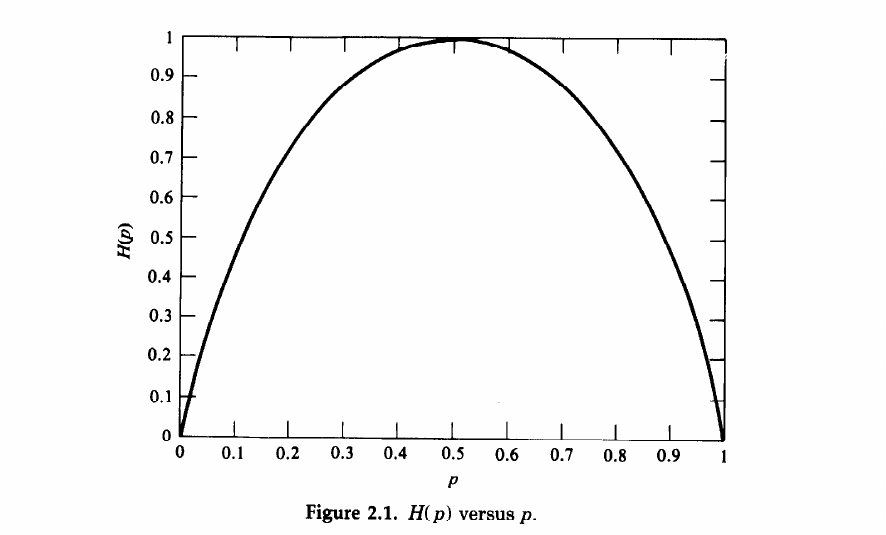
\includegraphics[width=.5\columnwidth]{coverHp}
      \caption{credit: Thomas \& Cover}
      \end{figure}
     \item Let $X=\begin{cases}a&\textnormal{w.p. }\frac{1}{2}\\b&\textnormal{w.p. }\frac{1}{4}\\c&\textnormal{w.p. }\frac{1}{8}\\d&\textnormal{w.p. }\frac{1}{8}\\ \end{cases}$ then
                   $$\Ent{X}=\frac{7}{4} (bits)$$
      \textbf{Optimal Source Coding (Huffman)}: Let a code be $a\to 0$, $b\to 10$, $c\to 110$, $d\to 111$, then the avg. message length is
      $$1\frac{1}{2}+2\frac{1}{4}+3\frac{1}{8}+3\frac{1}{8}=\frac{7}{4} (bits)$$
                   
    \end{itemize}
}
\frame{\frametitle{Diferential Entropy}
    \begin{definition}
    The \textbf{diferential entropy} of a r.v. $X$ with a probability density function $f(x)$ defined over a \textit{continuous} support set $x\in\mathcal{X}$ is
    \begin{equation}
     h(X)=-\Ex{X}{\log(p(x))}=-\int_{x\in\mathcal{X}}p(x)\log(p(x))
    \end{equation}
    \end{definition}
    \begin{itemize}
     \item \textcolor{ARust}{$\cancel{h(X)\geq 0}$}
     \item Careful with $+C$ in the integral!
    \end{itemize}
    \begin{theorem}
     Among all random variables with support in $\mathcal{X}=\mathbb{R}$, zero mean and variance $\sigma^2$, the entropy is maximized if $X$ is Gaussian
     \begin{equation}
      \begin{split}
       \max_{f(x)}&\; h(x)\\ \;\textnormal{s.t. }&\Ex{X}{x}=0\textnormal{ and } \Ex{X}{x^2}=\sigma^2
      \end{split} \Leftrightarrow \mathcal{N}(0,\sigma^2)
     \end{equation}
    \end{theorem}
}

\frame[allowframebreaks]{\frametitle{Entropy of Multiple Variables}
    \begin{definition}
    The \textbf{joint entropy} of a pair of r.v. $(X,Y)$ is
     $$\Ent{X,Y}=-\sum_{(x,y)\in\mathcal{X}\times\mathcal{Y}}p(x,y)\log(p(x,y))$$
    \end{definition}
    \begin{itemize}
     \item Complex numbers $z \triangleq (\Re\{z\},\Im\{z\})$
     \item Vectors $\x\in \mathbb{C}^N \triangleq (x_1,x_2,\dots x_N)$
    \end{itemize}
    \begin{theorem}
     Among and random variables $X$ with support in $\mathbb{C}^N$, zero mean and covariance matrix $\Sg$, the entropy is maximized if $X$ is $\mathcal{CN}(0,\Sg)$
     \end{theorem}
     \begin{remark}[p.d.f. of $\mathcal{CN}(\vec{\mu},\Sg)$]
        $f(\x)=\pi^{-N}\det(\Sg)^{-1}e^{-(\x-\vec\mu)^H\Sg^{-1}(\x-\vec\mu)}$
     \end{remark}


     \pagebreak
    \begin{definition}
    The \textbf{conditional entropy} of r.v. $X$ conditioned on $Y$ is    
     $$\CEnt{X}{Y}=\Ex{p(y)}{\Ent{X|Y=y}}=-\sum_{(x,y)\in\mathcal{X}\times\mathcal{Y}}\textcolor{ARust}{p(x,y)}\log(p(x|Y=y))$$
    \end{definition}
    \begin{theorem}[Chain Rule]
        $$\Ent{X,Y}=\Ent{X}+\CEnt{Y}{X}$$
    \end{theorem}
    \begin{theorem}[Conditioning Reduces Entropy]
        $$\Ent{X}\geq\CEnt{X}{Y}$$
    \end{theorem}
}
\frame[allowframebreaks]{\frametitle{Measuring Information}
    \begin{definition}
        The \textbf{mutual information} between two r.v. $X$ and $Y$ is
        $$\Inf{X}{Y}=\Ent{X}-\CEnt{X}{Y}=\int_x\int_yf(x,y)\log\left(\frac{f(x,y)}{f(x)f(y)}\right)$$
    \end{definition}
    ``How much uncertainty of $X$ decreases if we know $Y$''
    
    \begin{theorem}[Shannon’s channel coding theorem]
        For dependent r.v. $Y$ as a function of r.v. $X$, the \textbf{capacity}, defined as the maximum rate of ``reliable'' communication through the channel $f(Y|X)$, is
        $$C=\sup_{f(x)} \Inf{X}{Y}\textnormal{  s.t.  (constraints)}$$
    \end{theorem}
    
     \begin{figure}
      \centering
        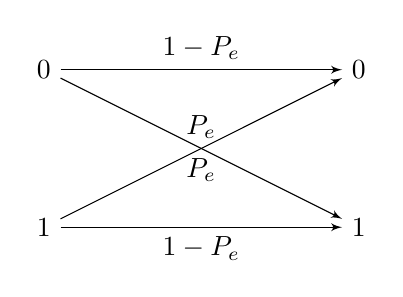
\begin{tikzpicture}[auto, node distance=4cm,>=latex']
            \node [pinstyle] (t0) {$0$};
            \node [pinstyle,below of=t0, node distance=2cm] (t1) {$1$};
            \node [pinstyle,right of=t0] (r0) {$0$};
            \node [pinstyle,right of=t1] (r1) {$1$};
            \draw[->] (t0) -- node[]{$1-P_e$} (r0);
            \draw[->] (t1) -- node[anchor=north]{$1-P_e$} (r1);
            \draw[->] (t0) -- node[anchor=north]{$P_e$} (r1);
            \draw[->] (t1) -- node[anchor=south]{$P_e$} (r0);
        \end{tikzpicture}
        \caption{Binary Simmetric Channel (BSC)}
     \end{figure}
     
     $$f(Y|X)\sim Y=\begin{cases}
                                               X&\textnormal{w.p. } 1-P_e\\
                                               \textnormal{not}(X)&\textnormal{w.p. } P_e
                                              \end{cases}\textnormal{ s.t. }X\in\{0,1\}$$
     $$C_{BSC}=1-H(P_e)$$
     \pagebreak
     
     
\begin{figure}
 \centering
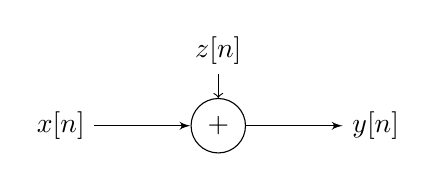
\begin{tikzpicture}[auto, node distance=2cm,>=latex']
    \node [pinstyle,anchor=east] (txin) {$x[n]$};
    \node [sum, right of=txin, node distance=2cm, pin={[pinstyle, pin distance=.3cm]above:$z[n]$}] (sum) {$+$};
    \draw [->,] (txin) -- (sum);
    \node [pinstyle, right of=sum] (rxout) {$y[n]$};
    \draw [->] (sum) -- (rxout);
\end{tikzpicture}
\caption{Additive White Gaussian Noise (AWGN) real channel}
\end{figure}
     $$y[n]=x[n]+z[n],\;\textnormal{ s.t. }z\sim\mathcal{N}(0,\sigma^2),\;x\in\mathbb{R},\;\Ex{}{|x|^2}=P$$
     $$C_{AWGN}=\frac{1}{2}\log\left(1+\frac{P}{\sigma^2}\right)\textnormal{ bits per channel use}$$
}

\frame[allowframebreaks]{\frametitle{Complex AWGN SISO DEC}

\begin{figure}
 \centering
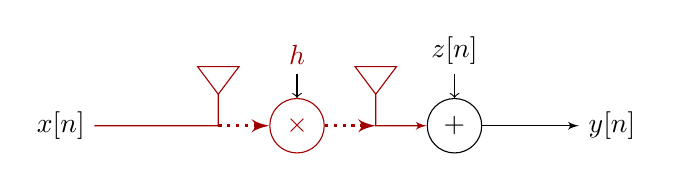
\begin{tikzpicture}[auto, node distance=2cm,>=latex']
    \node [pinstyle] (tx) {$x[n]$};
    \node [output,right of=tx] (txant) {};
    \draw [-,ARust] (tx) -- (txant) \antenna;
    \node [sum,color=ARust, right of=txant, pin={[pinstyle, pin distance=.3cm,color=ARust]above:$h$}] (mult) {$\times$};
    \node [input,right of=mult] (rxant) {};
    \draw [->,dotted,very thick,ARust] (txant) -- (mult);
    \draw [->,dotted,very thick,ARust] (mult) -- (rxant);
    \node [sum, right of=rxant, pin={[pinstyle, pin distance=.3cm]above:$z[n]$}] (sum) {$+$};
    \draw [->,ARust] (rxant) \antenna -- (sum) ;
    \node [pinstyle, right of=sum] (rec) {$y[n]$};
    \draw [->] (sum) -- (rec);
\end{tikzpicture}
 \caption{AWGN SISO Discrete Equivalent Channel}
\end{figure}
 $$y[n]=h·x[n]+z[n],\;z[n]\sim\mathcal{CN}(0,\sigma^2),\;x[n]\in\mathbb{C}\;\Ex{}{|x[n]|^2}=P$$
 $$C=B\log\left(1+\frac{|h|^2P}{\sigma^2}\right) \textnormal{ (bps)}$$
\begin{itemize}
 \item Bandwidth in Hertz $B$ (complex baseband or real passband $T_s\leq 2B$)
 \item \textbf{Received} SNR $\frac{|h|^2P}{\sigma^2}$
\end{itemize}

\pagebreak
\begin{definition}[Spectral Efficiency]
 Ratio between the communication rate and the employed bandwidth $\eta\triangleq \frac{R}{B}$
\end{definition}

  $$\eta_{\max}=\frac{C}{B}=\log\left(1+\frac{|h|^2P}{\sigma^2}\right)$$
  \begin{itemize}
    \item S.E. only grows logarithmically with SNR\\ \ \\
    \item $C$ grows linearly with $B$, but spectrum licenses are \textbf{very} expensive\\ \ \\
    \item What technology can increase S.E. efficiently?
  \end{itemize}
}

\frame[allowframebreaks]{\frametitle{Complex AWGN MIMO DEC}

\begin{figure}
 \centering
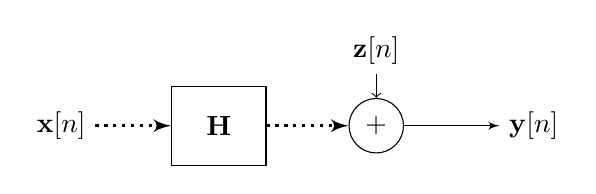
\begin{tikzpicture}[auto, node distance=2cm,>=latex']
    \node [pinstyle] (tx) {$\x[n]$};
    \node [block,right of=tx] (mult) {$\Hb$};
    \draw [->,dotted,very thick] (tx) -- (mult);
    \node [sum, right of=mult, node distance=2cm, pin={[pinstyle, pin distance=.3cm]above:$\z[n]$}] (sum) {$+$};
    \draw [->,dotted,very thick] (mult) -- (sum);
    \node [pinstyle, right of=sum] (rec) {$\y[n]$};
    \draw [->] (sum) -- (rec);
\end{tikzpicture}
 \caption{ \textbf{AWGN MIMO Discrete Equivalent Channel} (omit notation $[n]$)}
\end{figure}

    $$\y=\Hb\x+\z$$
        
\begin{columns}
\begin{column}{6cm}
    \begin{figure}
    \includesvg[width=\columnwidth]{channel}
    \end{figure}
\end{column}
\begin{column}{6cm}
    $\Hb=\left(\begin{array}{cccc}
 h_{1,1}&\dots&h_{1,N_{t}}\\
 \vdots&\ddots&\vdots\\
 h_{N_{r},1}&\dots&h_{N_{r},N_{t}}\\
\end{array}\right)
$
\end{column}
\end{columns}
 \begin{itemize}
 \item Number of transmit and receive antennas $N_{t}$, $N_{r}$
 $$\x\in \mathbb{C}^{N_{t}},\;\Hb\in \mathbb{C}^{N_{r}\times N_{t}},\;\y,\z\in \mathbb{C}^{N_{r}},\;$$
 \item Total transmitted power constraint (embedded in un-normalized $f(\x)$)
 $$\Ex{}{\sum_{i=1}^{N_{t}}|x_i[n]|^2}=\Ex{}{\|\x\|^2}=\Ex{}{\x^H\x}\leq P$$
 \item Transmitted signal covariance $\Ex{}{\x\x^H}=\Sg_{\x}$
 $$\underset{\textnormal{tr circular rotation identity}}{\underbrace{\tr{\A\B\Cb}=\tr\{\Cb\A\B\}}}\Rightarrow \Ex{}{\x^H\x}=\Ex{}{\tr\{\x\x^H\}}=\tr\{\Sg_{\x}\}\leq P$$
 \pagebreak
 \item Additive White Gaussian Noise $\Ex{}{\z\z^H}=\Sg_{\z}=\sigma^2\I$
 \begin{itemize}
    \item Suppose Thermal Noise of PSD $N_o\to\sigma^2=BN_o$\\ \ \\
 \end{itemize} 
 \item What if $x_i=\sqrt{\frac{P}{N_{t}}}s_i$ where $s_i$ are i.i.d. constellations?
 \begin{itemize}
    \item Input covariance $\Sg_\x=\frac{P}{N_{t}}\I_{N_{t}}$
    \item Received Signal Power $\tr\{\Hb\Sg_\x\Hb^H\}=\frac{P}{N_{t}}\tr\{\Hb\Hb^H\}=\frac{P}{N_{t}}\sum_{i,j=1}^{N_{t},N_{r}} |h_{i,j}|^2=\frac{P\|\Hb\|^2}{N_{t}}$
    \item Noise Power $\tr\{\Sg_\z\}=N_{r}\sigma^2$
    \item Receiver SNR $\frac{P\|\Hb\|^2}{N_{t}N_{r} \sigma^2}$\\ \ \\
 \end{itemize} 
 \item Normalized Channel Matrix $\|\Hb\|^2=N_{t}N_{r}\to$ SNR (of i.i.d. inputs) $=\frac{P}{\sigma^2}$ \\ \ \\
 \item \textbf{In this DEC, $P$ [Joules] energy received (w. pathloss), $\frac{P}{T_s}=PB$ [Watts]}
\end{itemize}
}

\frame[allowframebreaks]{\frametitle{AWGN MIMO Mutual Information}
\begin{itemize}
 \item Capacity is the maximum M.I. over all input distributions
 $$C\triangleq \max_{f(\x)} \Inf{\x}{\y}$$
 \item Gaussian $\y$ maximizes M.I. over all cases with $\Sg_\y=\Hb\Sg_\x\Hb^H+\Sg_\z$
    $$\Inf{\x}{\y}=\underset{\textnormal{max if }\y\textnormal{ is Gaussian}}{\underbrace{\Ent{\y}}}-\underset{\y|\x \sim  \mathcal{CN}(\Hb\x,\sigma^2\I)\textnormal{ always } \forall f(\x)}{\underbrace{\CEnt{\y}{\x}}}$$
 \item If $\x$ is Gaussian, so is $\y=\Hb\x+\z$
 \item Gaussian $\vv$ p.d.f. $f(\vv)=\pi^{-N}\det(\Sg_\vv)^{-1}e^{-(\vv-\vec\mu)^H\Sg_\vv^{-1}(\vv-\vec\mu)}$
 $$C= \max_{\Sg_\x} \Inf{\x}{\y} \big|_{\x\sim \mathcal{CN}(0,\Sg_\x)} = \max_{\Sg_\x}\log\det \left(\I_{N_{r}}+\Sg_\z^{-1}\Hb\Sg_\x\Hb^H\right)$$
\end{itemize}

What about optimization constraints?
 $$C= \max_{\Sg_\x}\log\det \left(\I_{N_{r}}+\frac{1}{\sigma^2}\Hb\Sg_\x\Hb^H\right)\textnormal{ s.t. \textcolor{ARust}{????????}}$$
 \begin{itemize}
  \item Total average transmitted power $\tr\{\Sg_\x\}\leq P$?
  \item RF power amplifier in each antenna $x_i\leq P/N_{t}\forall i$?
  \item Does the receiver know $\Hb$?
  \item Does the transmitter know $\Hb$? 
 \end{itemize}
 
 \begin{definition}[$C$ with only Channel State Information at the Receiver]
    $$C_{\textnormal{CSIR}}= \max_{\Sg_\x}\log\det \left(\I_{N_{r}}+\frac{1}{\sigma^2}\Hb\Sg_\x\Hb^H\right)\textnormal{ s.t. }\tr\{\Sg_\x\}\leq P, \Sg_x\textnormal{ const. }\forall \Hb$$
 \end{definition}
 \begin{definition}[$C$ with Channel State Information at the Transmitter]
    $$C_{\textnormal{CSIT}}= \max_{\Sg_\x}\log\det \left(\I_{N_{r}}+\frac{1}{\sigma^2}\Hb\Sg_\x\Hb^H\right)\textnormal{ s.t. }\tr\{\Sg_\x\}\leq P, \Sg_x=\mathscr{F}(\Hb)$$
 \end{definition}

}

\frame[allowframebreaks]{\frametitle{AWGN MIMO CSIR Capacity}
    \begin{itemize}
     \item No reason to transmit more power in one antenna than other
     \item No reason to transmit more power in \textit{algebraic} direction than other
    \begin{theorem}[M.I. Unitary Transform]
     For any unitary matrix $\U$, the channels $\y=\Hb\x+\z$ and $\y=\Hb'\x'+\z$ with $\Hb'=\Hb\U^H$, $\x'=\U\x$ have equal output and capacity $\Inf{\y}{\x}=\Inf{\y}{\U\x}$.
    \end{theorem}
    \item so we choose the input covariance $\Sg_\x= \frac{P}{N_{t}}\I_{N_{t}}$
    $$C_{\textnormal{CSIR}}= \log\det \left(\I_{N_{r}}+\frac{P}{N_{t}\sigma^2}\Hb\Hb^H\right)$$
    \end{itemize}
}

\frame[allowframebreaks]{\frametitle{Channel Eigenvalue Decomposition}
    \begin{itemize}
     \item $\Hb\Hb^H$ is square $N_{r}\times N_{r}$, admits \textit{eigenvalues} analysis
     \item $\Hb\Hb^H$ is Hermitian
     \begin{itemize}
        \item Non-negative eigenvalues $\lambda_1\geq \lambda_2\geq\dots\geq\lambda_{N_{r}}\geq 0$
        \item Decompositoin $\Hb\Hb^H=\U\Ld\U^H$
        $$\U^H\U=\U^H\U=\I,\;\Ld_{N_{r}}=\left(\begin{array}{cccc}
 \lambda_1&0&\dots&0\\
 0&\lambda_2&\dots&0\\
 \vdots&\vdots&\ddots&\vdots\\
 0&0&\dots&\lambda_{N_{r}}\\
\end{array}\right)$$
     \end{itemize}
    \end{itemize}
    \begin{equation*}
     \begin{split}
      C&=\log\det \left(\I_{N_{r}}+\frac{P}{N_{t}\sigma^2}\Hb\Hb^H\right)=\log\cancel{\det(\U)}^{1}\det\left(\I_{N_{r}}+\frac{P}{N_{t}\sigma^2}\Ld\right)\cancel{\det(\U^H)}^{1}\\
       &=\log\prod_{j=1}^{N_{r}} (1+\frac{P}{N_{t}\sigma^2}\lambda_j)=\sum_{j=1}^{N_{r}}\log (1+\frac{P}{N_{t}\sigma^2}\lambda_j)
     \end{split}
    \end{equation*}

\pagebreak
     \begin{definition}[Rank]
        Number of non-zero eigenvalues $\rank(\Hb) \triangleq \mathrm{count}(|\lambda_i|\neq0)\leq \min(N_{r},N_{t})$
     \end{definition}
     \begin{definition}[Eigenchannels]
      The MIMO capacity is the sum of $\rank(\Hb)$ SISO channel with gains $\lambda_i$
     \end{definition}
     \begin{figure}
        \centering
        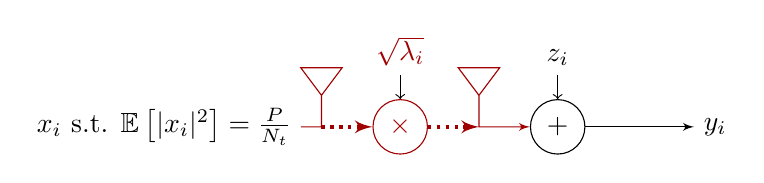
\begin{tikzpicture}[auto, node distance=2cm,>=latex']
            \node [pinstyle] (tx) {$x_i$ s.t. $\Ex{}{|x_i|^2}=\frac{P}{N_{t}}$};
            \node [output,right of=tx] (txant) {};
            \draw [-,ARust] (tx) -- (txant) \antenna;
            \node [sum,color=ARust, right of=txant, pin={[pinstyle, pin distance=.3cm,color=ARust]above:$\sqrt{\lambda_i}$}] (mult) {$\times$};
            \node [input,right of=mult] (rxant) {};
            \draw [->,dotted,very thick,ARust] (txant) -- (mult);
            \draw [->,dotted,very thick,ARust] (mult) -- (rxant);
            \node [sum, right of=rxant, pin={[pinstyle, pin distance=.3cm]above:$z_i$}] (sum) {$+$};
            \draw [->,ARust] (rxant) \antenna -- (sum) ;
            \node [pinstyle, right of=sum] (rec) {$y_i$};
            \draw [->] (sum) -- (rec);
        \end{tikzpicture}
        \caption{AWGN SISO Discrete Equivalent Channel}
        \end{figure}
    $$C=\sum_{j=1}^{\rank(\Hb)}C_i^{SISO}=\sum_{j=1}^{\rank(\Hb)}\log(1+\frac{P\lambda_i}{N_{t}\sigma^2})$$
\pagebreak
    \begin{itemize}
     \item $\|\Hb\|^2=\sum_{i,j=1}^{N_{t},N_{r}} |h_{i,j}|^2=\sum_{j=1}^{N_{r}}\lambda_j$
     \item Best case scenario: $N_{t}=N_{r}=N$, $\lambda_i=\lambda$, $\|\Hb\|^2=\sum_{j=1}^{N_{r}}\lambda_j=N\lambda=N^2$
     $$C=\textcolor{ARust}{N}\log(1+\frac{P}{\sigma^2})$$
    \begin{itemize}
     \item Capacity grows \textbf{linearly} with $N$\\ \ \\
     \end{itemize}
\pagebreak
     \item Least favorable scenario: $\rank(\Hb)=1$, $\lambda_1=N_{t}N_{r}=\|\Hb\|^2$
     $$C=\log(1+\frac{P\cancel{N_{t}}\textcolor{ARust}{N_{r}}}{\cancel{N_{t}}\sigma^2})$$
    \begin{itemize}
     \item Receive-only \textbf{MRC array gain}\\ \ \\
     \end{itemize}
     \item \textbf{SIMO only scales logarithmically}
     \item \textbf{MISO does not increase $C_{\textnormal{CSIR}}$ at all!}
     \end{itemize}
}

\frame[allowframebreaks]{\frametitle{AWGN MIMO CSIT Capacity}
\begin{itemize}
 \item Singular Value Decomposition of $\Hb=\U\Ld^{\frac{1}{2}}\V^H$
        $$\small \U^H\U=\I_{N_{r}},\;\V^H\V=\I_{N_{t}},\;\Ld^{\frac{1}{2}}=\left(\begin{array}{cccc}
 \sqrt{\lambda_1}&0&\dots&0\\
 0&\sqrt{\lambda_2}&\dots&0\\
 \vdots&\vdots&\ddots&\vdots\\
 0&0&\dots&\sqrt{\lambda_{\rank(\Hb)}}\\
\end{array}\right),\;\Ld_{\rank(\Hb)}=(\Ld^{\frac{1}{2}})^H\Ld^{\frac{1}{2}}$$
 \item Introduce the change of variable $\x=\V\x'$
 
\begin{figure}
 \centering
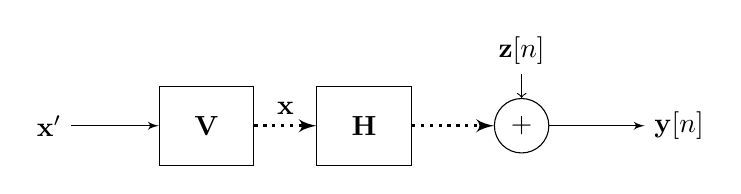
\begin{tikzpicture}[auto, node distance=2cm,>=latex']
    \node [pinstyle] (tx) {$\x'$};
    \node [block,right of=tx] (precod) {$\V$};
    \draw [->] (tx) -- (precod);
    \node [block,right of=precod] (mult) {$\Hb$};
    \draw [->,dotted,very thick] (precod) -- node {$\x$} (mult);
    \node [sum, right of=mult, node distance=2cm, pin={[pinstyle, pin distance=.3cm]above:$\z[n]$}] (sum) {$+$};
    \draw [->,dotted,very thick] (mult) -- (sum);
    \node [pinstyle, right of=sum] (rec) {$\y[n]$};
    \draw [->] (sum) -- (rec);
\end{tikzpicture}
 \caption{AWGN MIMO DEC with linear tx. precoding}
\end{figure}
 \item Covariance of channel input $\Sg_\x=\V\Sg_{\x}'\V^H$
 \item $\Sg_\x$ and $\Sg_{\x}'$ square, $\V$ is unitary $\to$ bijective projection of optimal $\Sg_{\x}'$
\end{itemize}
 \begin{theorem}[Sylverster's Theorem]
  For any matrices $\A\in\mathbb{C}^{n,m},\B\in\mathbb{C}^{m,n}$, $\det(\I_n+\A\B)=\det(\I_m+\B\A)$
 \end{theorem}
 \begin{equation*}
  \begin{split}
    C_{\textnormal{CSIT}}%&= \max_{\Sg_\x}\log\det \left(\I_{N_{r}}+\frac{1}{\sigma^2}\Hb\Sg_\x\Hb^H\right)\\
                         &= \max_{\Sg_\x}\log\det \left(\I_{N_{r}}+\frac{1}{\sigma^2}\U\Ld^{\frac{1}{2}}\V^H\Sg_\x\V(\Ld^{\frac{1}{2}})^H\U^H\right)\\
                         &= \max_{\Sg_\x'}\log\det \left(\I_{N_{r}}+\frac{1}{\sigma^2}\underset{\A}{\underbrace{\U\Ld^{\frac{1}{2}}}}\underset{\B}{\underbrace{\Sg_{\x'}(\Ld^{\frac{1}{2}})^H\U^H}}\right)\\
                         &= \max_{\Sg_\x'}\log\det \left(\I_{N_{r}}+\frac{1}{\sigma^2}\Sg_{\x'}(\Ld^{\frac{1}{2}})^H\U^H\U\Ld^{\frac{1}{2}}\right)\\
                         &= \max_{\Sg_\x'}\log\det \left(\I_{N_{r}}+\frac{1}{\sigma^2}\Sg_{\x'}\Ld_{\rank(\Hb)}\right)\\
  \end{split}
 \end{equation*}
 \pagebreak
 \begin{theorem}[Hadamard Inequality]
  For any non-negative definite matrix $\A$, $\det(\A)\leq \prod A_{i,i}$ where $A_{i,i}$ are the diagonal elements of $\A$. Equality is achieved with diagonal $\A$.
 \end{theorem}
 \begin{itemize}
  \item There is at least one optimal $\Sg_{\x'}$ that is diagonal
 \end{itemize}
\begin{columns}
 \begin{column}{6cm}
  $$\D_{\x'}=\left(\begin{array}{cccc}
 P_1&0&\dots&0\\
 0&P_2&\dots&0\\
 \vdots&\vdots&\ddots&\vdots\\
 0&0&\dots&P_{\rank(\Hb)}\\
\end{array}\right)$$  
 \end{column}
 \begin{column}{6cm}
 \begin{equation*}
  \begin{split}
    C_{\textnormal{CSIT}}&= \max_{\D_\x'}\log\det \left(\I_{N_{r}}+\frac{1}{\sigma^2}\D_{\x'}\Ld\right)\\
        &= \max_{(P_1,P_2,\dots,P_{r_\Hb})}\log\prod_{i=1}^{\rank(\Hb)} \left(1+\frac{P_i\lambda_i}{\sigma^2}\right)\\
        &= \max_{(P_1,P_2,\dots,P_{r_\Hb})}\sum_{i=1}^{\rank(\Hb)}\log \left(1+\frac{P_i\lambda_i}{\sigma^2}\right)\\
  \end{split}
 \end{equation*}
 \end{column}
\end{columns}
}

\frame{\frametitle{Eigenbeamforming}
\begin{figure}
 \centering
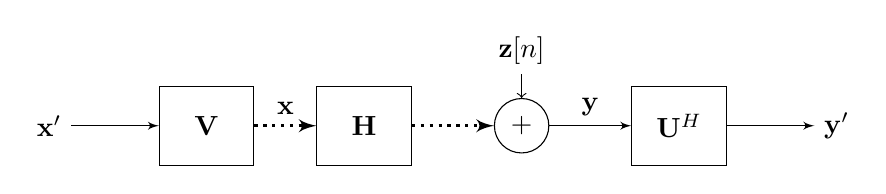
\begin{tikzpicture}[auto, node distance=2cm,>=latex']
    \node [pinstyle] (tx) {$\x'$};
    \node [block,right of=tx] (precod) {$\V$};
    \draw [->] (tx) -- (precod);
    \node [block,right of=precod] (mult) {$\Hb$};
    \draw [->,dotted,very thick] (precod) -- node {$\x$} (mult);
    \node [sum, right of=mult, node distance=2cm, pin={[pinstyle, pin distance=.3cm]above:$\z[n]$}] (sum) {$+$};
    \draw [->,dotted,very thick] (mult) -- (sum);
    \node [block,right of=sum] (decod) {$\U^H$};
    \draw [->] (sum) -- node {$\y$} (decod);
    \node [pinstyle, right of=decod] (rec) {$\y'$};
    \draw [->] (decod) -- (rec);
\end{tikzpicture}
 \caption{AWGN MIMO DEC CSIT Eigenbeamforming}
\end{figure}
\begin{itemize}
 \item Transmitter linear precoding $\x=\V\x'$
 \item Receiver linear combining $\y'=\U^H\y$
 \end{itemize}
 
\begin{columns}
 \begin{column}{6cm}
\begin{figure}
 \centering
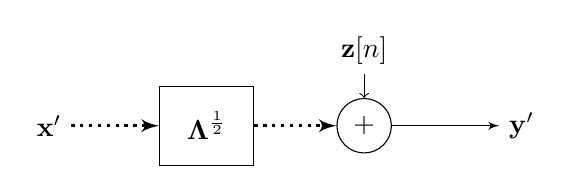
\begin{tikzpicture}[auto, node distance=2cm,>=latex']
    \node [pinstyle] (tx) {$\x'$};
    \node [block,right of=tx] (mult) {$\Ld^{\frac{1}{2}}$};
    \draw [->,dotted,very thick] (tx) -- (mult);
    \node [sum, right of=mult, node distance=2cm, pin={[pinstyle, pin distance=.3cm]above:$\z[n]$}] (sum) {$+$};
    \draw [->,dotted,very thick] (mult) -- (sum);
    \node [pinstyle, right of=sum] (rec) {$\y'$};
    \draw [->] (sum) -- (rec);
\end{tikzpicture}
 \caption{Eigenchannels}
\end{figure}  
 \end{column}
 \begin{column}{6cm}
      $$C_{\textnormal{CSIT}}=\max_{(P_1,P_2,\dots,P_{r_\Hb})}\sum_{i=1}^{\rank(\Hb)}\log \left(1+\frac{P_i\lambda_i}{\sigma^2}\right)$$
 \end{column}
\end{columns}
}


\frame[allowframebreaks]{\frametitle{Waterfilling}
    \begin{itemize}
     \item What is the optimal allocation of power to Eigenchannels?\\ \ \\
     \item Convex optimization with constraints
     $$\max_{\vec{P}} f(\vec{P})\textnormal{ s.t. }\sum P_i=P,\; P_i>0\forall i$$ $$f(\vec{P})=\sum_{i=1}^{\rank(\Hb)}\log \left(1+\frac{P_i\lambda_i}{\sigma^2}\right)$$
     \item Lagrange Multipliers
     $$\max_{\vec{P}}\mathscr{L}(\vec{P})$$ $$\mathscr{L}(\vec{P}) = f(\vec{P})-\beta(\sum P_i-P)+\sum \zeta_i(P_i)$$
     \item Gradient of $\mathscr{L}(\vec{P})=\sum_{i=1}^{\rank(\Hb)}\underset{\ell_i(P_i)}{\underbrace{\left[\log \left(1+\frac{P_i\lambda_i}{\sigma^2}\right)-\beta P_i+\zeta_iP_i\right]}}+\beta P$
     \begin{equation*}\begin{split}
     0&=\frac{\partial \mathscr{L}(\vec{P})}{\partial P_i}= \frac{\partial \ell_i(P_i)}{\partial P_i} = \frac{ \lambda_i }{\sigma^2+P_i\lambda_i}-\beta+\zeta_i\\
    \beta-\zeta_i &= \frac{ \lambda_i }{\sigma^2+P_i\lambda_i}\\
    \sigma^2+P_i\lambda_i &= \frac{ \lambda_i }{\beta-\zeta_i}\\
    P_i &= \frac{ 1 }{\beta-\zeta_i}-\frac{\sigma^2}{\lambda_i}\\
    \end{split}
     \end{equation*}
    \item Condition $\zeta_iP_i^*=0\to$ for $P_i^*\neq 0, \zeta_i=0$
        $$P_i^* = \begin{cases}                 
                    \frac{ 1 }{\beta}-\frac{\sigma^2}{\lambda_i}&\textnormal{if }\frac{ 1 }{\beta}>\frac{\sigma^2}{\lambda_i}\\
                    0&\textnormal{otherwise}
                \end{cases}$$
    \item Condition $\beta (\sum P_i-P)=0\to$,  for $\beta\neq0, \sum P_i=P$     \\ \ \\
    \item Optimal power allocation Solution
     $$P_i^*=\left(\frac{1}{\beta}-\frac{\sigma^2}{\lambda_i}\right)^+\;\leftarrow \textnormal{ substitute in }\sum P_i^*=P \textnormal{ and calculate }\beta$$
    \end{itemize}
    
\begin{columns}
 \begin{column}{7cm}    
    \setbeamercolor{postit}{fg=EETblue,bg=EETblue!10}
    \begin{beamercolorbox}[wd=\textwidth]{postit}
%     \begin{algorithm}
%     \caption{WATER FILLING ALGORITHM}
     \begin{algorithmic}[0]
      \STATE Define $w=\frac{1}{\beta}$
      \STATE Initialize $w^{(0)}=\frac{\sigma^2}{\lambda_i}$, $P_i^{(0)}=0$
      \WHILE{ $\{n=0;\sum P_i^{(n)}<P, n++\}$ }
        \STATE $P_{unused}=P-\sum P_i^{(n)}$
        \STATE $w^{(n+1)}=w^{(n)}+\frac{P_{unused}}{\rank(\Hb)}$
        \STATE $P_i^{(n+1)}=\left(w^{(n+1)}-\frac{\sigma^2}{\lambda_i}\right)^+$
      \ENDWHILE
     \end{algorithmic}
    \end{beamercolorbox}
%     \end{algorithm}
\begin{itemize}
 \item Let $N_{\Hb}=\left|\{P_i^*>0\}\right|$
\end{itemize}

$$C_{\textnormal{CSIT}}=\sum_{i=1}^{N_{\Hb}}\log\left(\frac{\lambda_i}{\beta\sigma^2}\right)$$
\end{column}
 \begin{column}{6cm}
\begin{figure}[t]
\centering
\scalebox{.75}{
    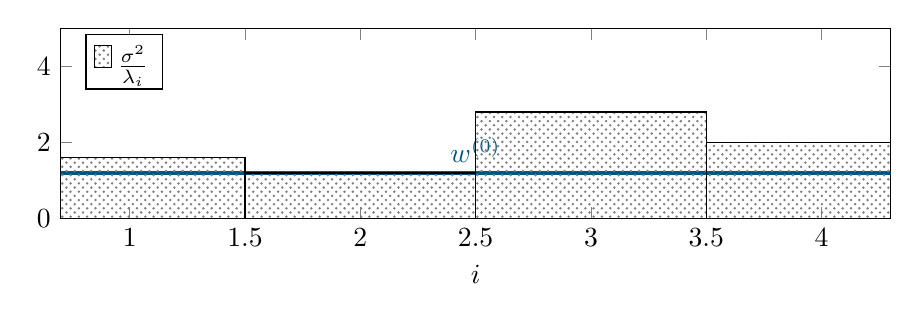
\begin{tikzpicture}[auto,>=latex']
        \begin{axis}[
        ybar stacked,
        width=\columnwidth,
        height=4cm,
        ymin=0,
        ymax=5,
%         xtick=1,
        legend style={
            cells={anchor=west},
            legend pos=north west,
        },
        reverse legend=true,
%         xticklabels = {1,2,3,4,5},
        xlabel={$i$},
        bar width=1,
    ]
        \addplot[draw=black,pattern color=gray,pattern=crosshatch dots] coordinates {
        (1,1.6)
        (2,1.2)
        (3,2.8)
        (4,2)
        };
    \draw[-,VCobalt,very thick] (0,1.2) -- node[VCobalt] {$w^{(0)}$} (5,1.2);
    \legend {$\frac{\sigma^2}{\lambda_i}$};
    \end{axis}
    \end{tikzpicture}
    }
    
\scalebox{.75}{
    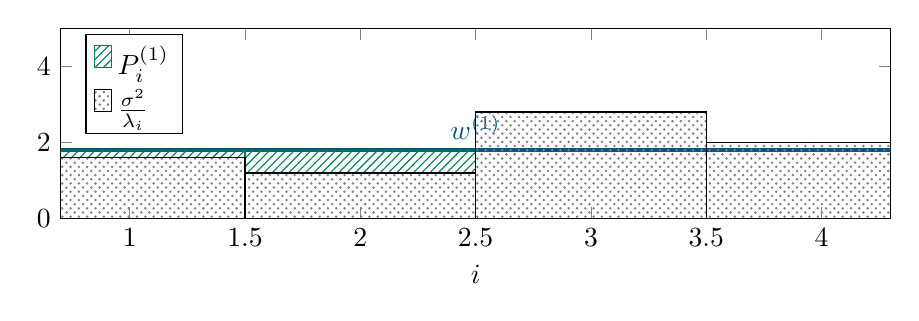
\begin{tikzpicture}[auto,>=latex']
        \begin{axis}[
        ybar stacked,
        width=\columnwidth,
        height=4cm,
        ymin=0,
        ymax=5,
%         xtick=1,
        legend style={
            cells={anchor=west},
            legend pos=north west,
        },
        reverse legend=true,
%         xticklabels = {1,2,3,4,5},
        xlabel={$i$},
        bar width=1,
    ]
        \addplot[draw=black,pattern color=gray,pattern=crosshatch dots] coordinates {
        (1,1.6)
        (2,1.2)
        (3,2.8)
        (4,2)
        };
        \addplot[draw=KYJade,pattern color=KYJade,pattern=north east lines] coordinates {
        (1,.2)
        (2,.6)
        (3,0)
        (4,)
        };
        \legend {$\frac{\sigma^2}{\lambda_i}$, $P_i^{(1)}$};
    \draw[-,VCobalt,very thick] (0,1.8) -- node[VCobalt] {$w^{(1)}$} (5,1.8);
    \end{axis}
    \end{tikzpicture}
    }
\scalebox{.75}{
    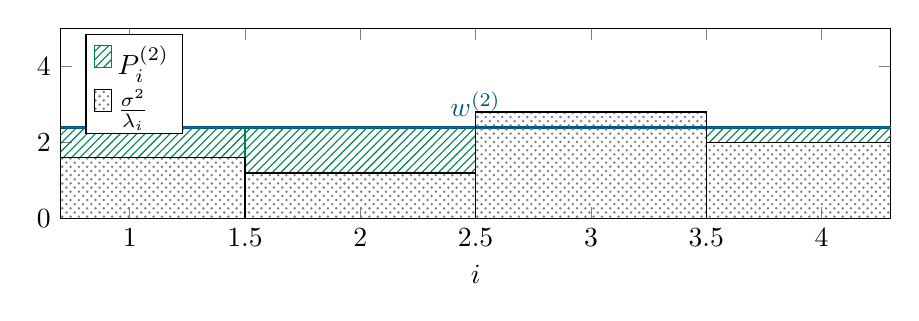
\begin{tikzpicture}[auto,>=latex']
        \begin{axis}[
        ybar stacked,
        width=\columnwidth,
        height=4cm,
        ymin=0,
        ymax=5,
%         xtick=1,
        legend style={
            cells={anchor=west},
            legend pos=north west,
        },
        reverse legend=true,
%         xticklabels = {1,2,3,4,5},
        xlabel={$i$},
        bar width=1,
    ]
        \addplot[draw=black,pattern color=gray,pattern=crosshatch dots] coordinates {
        (1,1.6)
        (2,1.2)
        (3,2.8)
        (4,2)
        };
        \addplot[draw=KYJade,pattern color=KYJade,pattern=north east lines] coordinates {
        (1,.8)
        (2,1.2)
        (3,0)
        (4,.4)
        };
        \legend {$\frac{\sigma^2}{\lambda_i}$, $P_i^{(2)}$};
    \draw[-,VCobalt,very thick] (0,2.4) -- node[VCobalt] {$w^{(2)}$} (5,2.4);
    \end{axis}
    \end{tikzpicture}
    }
\end{figure}    
 \end{column}
\end{columns}
}



\frame[allowframebreaks]{\frametitle{OFDM and MIMO Capacity}
%      \item With ISI, i.e. $\displaystyle \y=\sum_{m=0}^{M-1}\Hb[n-m]\x[m]+\z[m]$ with $M>1$\\ \ \\
 \begin{figure}
 \caption{OFDM frequency-selective channel split into $K$ flat sub-bands}
    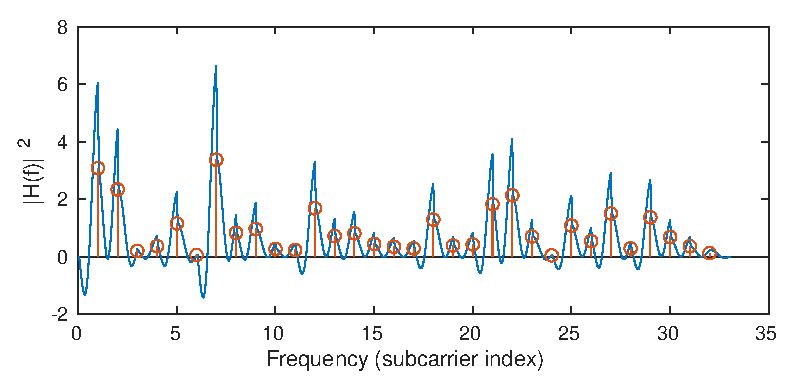
\includegraphics[width=.45\columnwidth]{ofdmexample} 
 \end{figure}
    \begin{itemize}
     \item Independent MIMO subchannels $\y[k]=\Hb[k]\x[k]+\z[k]\;\forall k\in[0,K-1]$
     \item ``stack'' the vectors as a large MIMO block-diagonal channel
         $$\Tiny \underset{\y_{tot}}{\underbrace{\left(\begin{array}{c}\y[0]\\\vdots\\\y[K-1]\end{array}\right)}}=\underset{\Hb_{tot}}{\underbrace{\left(\begin{array}{cccc}\Hb[0]&0&\dots&0\\ 0&\Hb[1]&\dots&0\\ \vdots&\vdots&\ddots&\vdots\\ 0&0&\dots&\Hb[K-1] \end{array}\right)}}\underset{\x_{tot}}{\underbrace{\left(\begin{array}{c}\x[0]\\\vdots\\\x[K-1]\end{array}\right)}}+\underset{\z_{tot}}{\underbrace{\left(\begin{array}{c}\z[0]\\ \vdots\\ \z[K-1]\end{array}\right)}}$$
  
%  \pagebreak
\item By M.I. chain rule and properties of block matrix, the capacity is
          \begin{equation}
            \begin{split}
                C&=\sup_{\Sg_{\x_{tot}}}\log\det\left(\I+\frac{1}{\sigma_z}\Hb_{tot}\Sg_{\x_{tot}}\Hb_{tot}^H\right)\\
                 &=\sup_{\{\Sg_{\x[k]}\}_{k=0}^{K-1}}\sum_{k=0}^{K-1}\log\det\left(\I+\frac{1}{\sigma_z}\Hb[k]\Sg_{\x[k]}\Hb^H[k]\right)\\
                 &=\sup_{\vec{P}}\sum_{k=0}^{K-1}\sum_{i=0}^{\rank(\Hb[k])}\log\left(1+\frac{P_{k,i}\lambda_i[k]}{\sigma_z}\right)
            \end{split}
          \end{equation}
     \item With CSIT, waterfilling over \textbf{antennas and frequency}
    \end{itemize}
}

\frame[allowframebreaks]{\frametitle{Degrees of Freedom}
\begin{columns}
\begin{column}{8cm}
\begin{figure}
 \centering
 \caption{Multipath Channel}
 \includesvg[width=.9\columnwidth]{multipath}
\end{figure}
\vspace{.1in}
\end{column}
\begin{column}{4cm}
\begin{itemize}
 \item System of Linear Equations
    $$\begin{array}{c}y_1=h_{1,1}x_1+h_{1,2}x_2\\y_2=h_{2,1}x_1+h_{2,2}x_2\end{array}$$    
 \item Has solution if $h_{1,1},h_{1,2},h_{2,1},h_{2,2}$ are all different
\end{itemize}
\end{column}
\end{columns}

Paradigm shift in interpretation of multipath channel
\begin{itemize}
 \item Before: ``multipath is a problem, creates Inter-Symbol Interference''
 \item Now: ``multipath is an opportunity, creates degrees of freedom''
\end{itemize}

\pagebreak
\begin{itemize}
 \item System of linear equations $\vv=\Hb\x$ has solution(s) if $\rank(\Hb)\stackrel{(>)}{=} N_{t}$
 \item How many independent modulation symbols can we send? Does the noise $\y=\vv+\z$ affect?
 \begin{definition}[Degrees of Freedom (DoF)]
  $$\textnormal{DoF}=\lim_{SNR_{norm}\to\infty}\frac{C}{\log(SNR_{norm})},\textnormal{ where }SNR_{norm}=\frac{P}{\sigma^2}$$
 \end{definition}
 \begin{theorem}
  If $\Hb$ is full rank, $D=\min(N_{t},N_{r})$
 \end{theorem}
\end{itemize}
}


\frame[allowframebreaks]{\frametitle{Energy Limited Rate}
\begin{itemize}
 \item Recall that $\sigma_z^2=BN_o$ and $C$ in bit/channel use
 $$C(bps)=\sup_{\vec{P}}B\sum_{i=1}^{\rank(\Hb)}\log\left(1+\frac{P_i\lambda_i}{N_oB}\right)$$
 \item The DoF reveal the \textit{PRELOG} of the big-O capacity scaling
 $$C\approx\Theta\left( B\min(N_{t},N_{r})\log\left(1+\frac{P}{N_oB}\frac{N_{t}N_{t}}{\min(N_{t},N_{r})}\right) \right)$$ 
 \item Spectral efficiency $\eta=\frac{C}{B}$ bits/s/Hz
 \item For small $B$, rate grows with DoF. 
    $$\eta \approx\Theta\left( \min(N_{t},N_{r})  \right)$$ 
 
 \pagebreak
 \item When bandwidth is very large
 $$\lim_{B\to\infty}C(bps)=\sup_{\vec{P}}B\frac{\sum_{i=1}^{\rank(\Hb)}P_i\lambda_i}{N_oB}\begin{cases}
                                                                                           \textnormal{CSIR }\to\frac{P\sum_{i=1}^{\rank(\Hb)}\lambda_i}{N_{t}N_oB}= \frac{P\|\Hb\|^2}{N_{t}N_oB}\\
                                                                                           \textnormal{CSIT }\to\frac{P\lambda_{\max}}{N_oB}\\
                                                                                          \end{cases}
$$
 \item The rate is limited by received energy, $\eta\to0$
 \begin{figure}
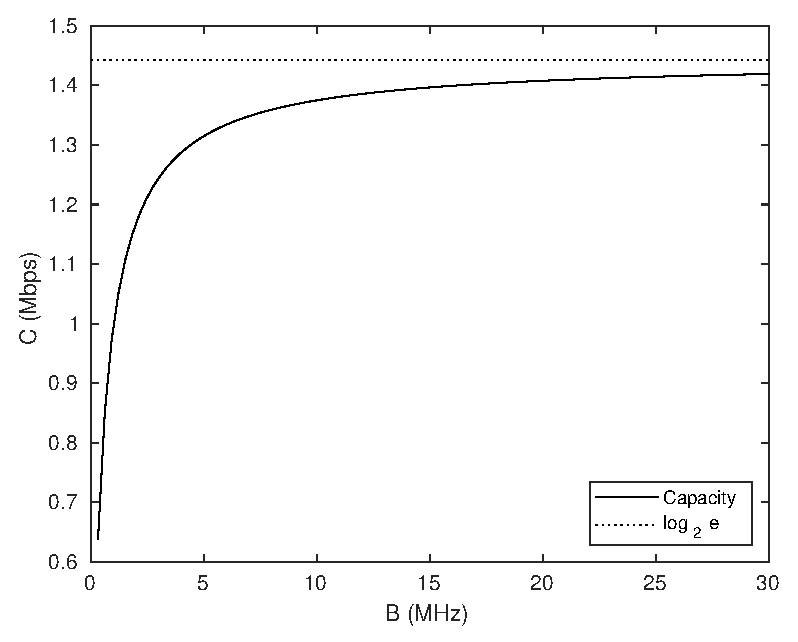
\includegraphics[width=.35\columnwidth]{widebandcap} 
\end{figure}

 \item Minimum energy per transmitted bit $\frac{P/N_o}{C_{SISO}}\geq -\log_2 e = -1.56dB$. \\ \ \\
\end{itemize}
}



\frame{\frametitle{Massive MIMO}
\begin{columns}
 \begin{column}{6cm}
 \textbf{Very large} number of antennas
  \begin{figure}
   \centering
   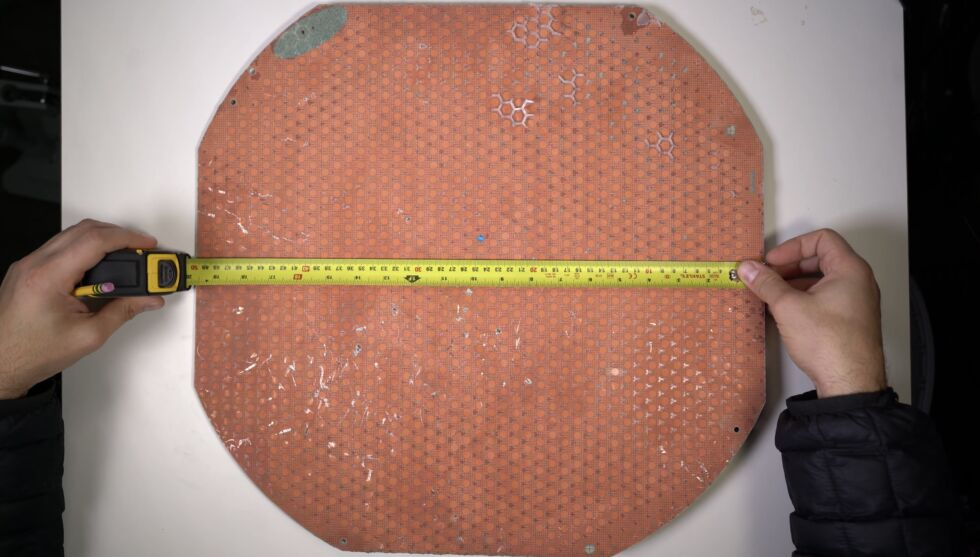
\includegraphics[width=\columnwidth]{starlink-24-phased-array-measurement-980x557}
   \caption{StarLink dish antennas\\https://www.youtube.com/watch?v=iOmdQnIlnRo}
  \end{figure}
 \end{column}
 \begin{column}{6cm}
 \begin{itemize}
    \item Advantages
    \begin{itemize}
        \item Unlimited capacity 
        $$ \lim_{N_{t},N_{r}\to\infty} C=\infty$$
        \item Random Matrix Theory
        $$\lim_{N_{t}\to\infty} \mathcal{CN}(0,\I_{N_{t}})\to U\textnormal{-sphere}$$\\ \ \\
    \end{itemize}
    \item Problems
    \begin{itemize}
        \item Hardware Complexity
        \item RF circuit power
        \item Channel Estimation
    \end{itemize}
 \end{itemize}
 \end{column}
\end{columns}

}
\end{document}


